\documentclass[11pt, a4paper]{article}\usepackage[]{graphicx}\usepackage[]{xcolor}
% maxwidth is the original width if it is less than linewidth
% otherwise use linewidth (to make sure the graphics do not exceed the margin)
\makeatletter
\def\maxwidth{ %
  \ifdim\Gin@nat@width>\linewidth
    \linewidth
  \else
    \Gin@nat@width
  \fi
}
\makeatother

\definecolor{fgcolor}{rgb}{0.345, 0.345, 0.345}
\newcommand{\hlnum}[1]{\textcolor[rgb]{0.686,0.059,0.569}{#1}}%
\newcommand{\hlsng}[1]{\textcolor[rgb]{0.192,0.494,0.8}{#1}}%
\newcommand{\hlcom}[1]{\textcolor[rgb]{0.678,0.584,0.686}{\textit{#1}}}%
\newcommand{\hlopt}[1]{\textcolor[rgb]{0,0,0}{#1}}%
\newcommand{\hldef}[1]{\textcolor[rgb]{0.345,0.345,0.345}{#1}}%
\newcommand{\hlkwa}[1]{\textcolor[rgb]{0.161,0.373,0.58}{\textbf{#1}}}%
\newcommand{\hlkwb}[1]{\textcolor[rgb]{0.69,0.353,0.396}{#1}}%
\newcommand{\hlkwc}[1]{\textcolor[rgb]{0.333,0.667,0.333}{#1}}%
\newcommand{\hlkwd}[1]{\textcolor[rgb]{0.737,0.353,0.396}{\textbf{#1}}}%
\let\hlipl\hlkwb

\usepackage{framed}
\makeatletter
\newenvironment{kframe}{%
 \def\at@end@of@kframe{}%
 \ifinner\ifhmode%
  \def\at@end@of@kframe{\end{minipage}}%
  \begin{minipage}{\columnwidth}%
 \fi\fi%
 \def\FrameCommand##1{\hskip\@totalleftmargin \hskip-\fboxsep
 \colorbox{shadecolor}{##1}\hskip-\fboxsep
     % There is no \\@totalrightmargin, so:
     \hskip-\linewidth \hskip-\@totalleftmargin \hskip\columnwidth}%
 \MakeFramed {\advance\hsize-\width
   \@totalleftmargin\z@ \linewidth\hsize
   \@setminipage}}%
 {\par\unskip\endMakeFramed%
 \at@end@of@kframe}
\makeatother

\definecolor{shadecolor}{rgb}{.97, .97, .97}
\definecolor{messagecolor}{rgb}{0, 0, 0}
\definecolor{warningcolor}{rgb}{1, 0, 1}
\definecolor{errorcolor}{rgb}{1, 0, 0}
\newenvironment{knitrout}{}{} % an empty environment to be redefined in TeX

\usepackage{alltt}

\usepackage[top = 1 in, bottom = 1 in, left = 1 in, right = 1 in ]{geometry}

\usepackage{amsmath, amssymb, amsfonts}
\usepackage{enumerate}
\usepackage{array}
\usepackage{multirow}
\usepackage{dingbat}
\usepackage{fontawesome5}
\usepackage{tasks}
\usepackage{bbding}
\usepackage{twemojis}
% how to use bull's eye ----- \scalebox{2.0}{\twemoji{bullseye}}
\usepackage{fontspec}
\usepackage{customdice}
% how to put dice face ------ \dice{2}

\title{MSMS 308 : Practical 04}
\author{Ananda Biswas \\[1em] Exam Roll No. : 24419STC053}
\date{\today}

\newfontface\myfont{Myfont1-Regular.ttf}[LetterSpace=0.05em]
% how to use ---- {\setlength{\spaceskip}{1em plus 0.5em minus 0.5em} \fontsize{17}{20}\myfont --write text here-- \par}

\newfontface\cbfont{CaveatBrush-Regular.ttf}
% how to use --- \myfont --write text here--
\IfFileExists{upquote.sty}{\usepackage{upquote}}{}
\begin{document}

\maketitle


\section*{\faArrowAltCircleRight[regular] \textcolor{blue}{Question}}

\hspace{1cm} Consider a lifetime variable that follows a \textbf{Weibull distribution} with shape parameter $\alpha$ and scale parameter $\lambda$. The probability density function of this distribution is given by:

\[
f(t; \alpha, \lambda) = \frac{\alpha}{\lambda} \left( \frac{t}{\lambda} \right)^{\alpha - 1} e^{-(t/\lambda)^\alpha}, \quad t > 0.
\]

Estimate the parameters by MLE and get respective Bias and Mean Squared Errors. Then plot the PDF, Survival Function, Hazard Function and Cumulative Hazard Function using the obtained estimates.

\section*{\faArrowAltCircleRight[regular] \textcolor{blue}{Build-up for obtaining MLE}}

For a sample of size $n$, the likelihood function is given by

\begin{align*}
L(\alpha, \lambda) &= \prod \limits_{i = 1}^{n} \frac{\alpha}{\lambda} \left( \frac{t_i}{\lambda} \right)^{\alpha - 1} e^{-(t_i / \lambda)^\alpha} \\
&= \left( \dfrac{\alpha}{\lambda} \right)^n \left( \prod \limits_{i = 1}^{n}  \dfrac{t_i}{\lambda} \right)^{\alpha - 1} \text{exp}\left\{- \sum \limits_{i = 1}^{n} \left( \dfrac{t_i}{\lambda}\ \right)^{\alpha} \right\}.
\end{align*}

\vspace{0.5cm}

The log-likelihood function is given by

$$l(\alpha, \lambda) = n \log \alpha - n \log \lambda + (\alpha - 1) \sum_{i=1}^{n} \log \left( \frac{t_i}{\lambda} \right) - \sum_{i=1}^{n} \left( \frac{t_i}{\lambda} \right)^{\alpha}.$$

Now, 
\begin{equation}
\dfrac{\partial}{\partial \alpha} l(\alpha, \lambda) = \dfrac{n}{\alpha} + \sum \limits_{i=1}^{n} \log \left( \dfrac{t_i}{\lambda} \right) - \sum \limits_{i=1}^{n} \left( \dfrac{t_i}{\lambda} \right)^{\alpha} \log \left( \dfrac{t_i}{\lambda} \right) = u(\alpha, \lambda) \text{, say}
\end{equation}

\newpage

and

\begin{align*}
\dfrac{\partial}{\partial \lambda} l(\alpha, \lambda) &= -\dfrac{n}{\lambda} + (\alpha - 1) \sum \limits_{i=1}^{n} \dfrac{\lambda}{t_i} \cdot \left( -\dfrac{t_i}{\lambda^2} \right) + \sum \limits_{i=1}^{n} \dfrac{\alpha \cdot t_i^{\alpha}}{\lambda^{\alpha + 1}}\\[0.3cm]
&= -\dfrac{n}{\lambda} - (\alpha - 1) \dfrac{n}{\lambda} + \sum \limits_{i=1}^{n} \dfrac{\alpha \cdot t_i^{\alpha}}{\lambda^{\alpha + 1}}\\[0.3cm]
&= -\dfrac{n \alpha}{\lambda} + \sum \limits_{i=1}^{n} \dfrac{\alpha \cdot t_i^{\alpha}}{\lambda^{\alpha + 1}} = v(\alpha, \lambda) \text{, say}.
\end{align*}

Setting $v(\alpha, \lambda) = 0$ we get,


\begin{align*}
-\dfrac{n \alpha}{\lambda} + \sum \limits_{i=1}^{n} \dfrac{\alpha \cdot t_i^{\alpha}}{\lambda^{\alpha + 1}} &= 0 \nonumber \\
\Rightarrow \dfrac{n}{\lambda} &= \sum \limits_{i=1}^{n} \dfrac{t_i^{\alpha}}{\lambda^{\alpha + 1}} \nonumber \\
\Rightarrow \dfrac{n}{\lambda} &= \dfrac{1}{\lambda^{\alpha + 1}} \sum \limits_{i=1}^{n}{t_i^{\alpha}} \nonumber \\
\Rightarrow \lambda^{\alpha} &= \dfrac{1}{n} \sum \limits_{i=1}^{n}{t_i^{\alpha}} \nonumber \\
\therefore \lambda &= \left( \dfrac{1}{n} \sum \limits_{i=1}^{n}{t_i^{\alpha}} \right)^{\frac{1}{\alpha}} \tag{2} \\
\end{align*}

\setcounter{equation}{2}


Setting $u(\alpha, \lambda) = 0$ does not yield any closed form solution. So for getting the ML estimate of $\alpha$, we resort to numerical methods (here Newton-Raphson method). \\[1em]

Now, 
\begin{equation}
u_{\alpha}(\alpha, \lambda) = \dfrac{\partial}{\partial \alpha} u(\alpha, \lambda) = -\dfrac{n}{\alpha^2} - \sum \limits_{i=1}^{n} \left( \dfrac{t_i}{\lambda} \right)^{\alpha} \left[ \log \left( \dfrac{t_i}{\lambda} \right) \right]^2;\\[0.3cm]
\end{equation}

At each iteration, with the present value of $\alpha$ we calculate $\lambda$ by using $(2)$; then we use the obtained value of $\lambda$ in $(1)$ and $(3)$ to improve the estimate of $\alpha$ by Newton-Raphson method.

\section*{\faArrowAltCircleRight[regular] \textcolor{blue}{R Program}}

\begin{knitrout}
\definecolor{shadecolor}{rgb}{0.969, 0.969, 0.969}\color{fgcolor}\begin{kframe}
\begin{alltt}
\hldef{estimate_lambda} \hlkwb{<-} \hlkwa{function}\hldef{(}\hlkwc{s}\hldef{,} \hlkwc{alpha}\hldef{)} \hlkwd{mean}\hldef{(s}\hlopt{^}\hldef{alpha)}\hlopt{^}\hldef{(}\hlnum{1}\hlopt{/}\hldef{alpha)}
\end{alltt}
\end{kframe}
\end{knitrout}

\begin{knitrout}
\definecolor{shadecolor}{rgb}{0.969, 0.969, 0.969}\color{fgcolor}\begin{kframe}
\begin{alltt}
\hldef{u} \hlkwb{<-} \hlkwa{function}\hldef{(}\hlkwc{alpha}\hldef{,} \hlkwc{lambda}\hldef{,} \hlkwc{s}\hldef{)\{}

  \hldef{a} \hlkwb{<-} \hlkwd{length}\hldef{(s)} \hlopt{/} \hldef{alpha}

  \hldef{b} \hlkwb{<-} \hlkwd{sum}\hldef{(}\hlkwd{log}\hldef{(s} \hlopt{/} \hldef{lambda))}

  \hldef{c} \hlkwb{<-} \hlkwd{sum}\hldef{((s} \hlopt{/} \hldef{lambda)}\hlopt{^}\hldef{alpha} \hlopt{*} \hlkwd{log}\hldef{(s} \hlopt{/} \hldef{lambda))}

  \hlkwd{return}\hldef{(a} \hlopt{+} \hldef{b} \hlopt{-} \hldef{c)}
\hldef{\}}
\end{alltt}
\end{kframe}
\end{knitrout}


\begin{knitrout}
\definecolor{shadecolor}{rgb}{0.969, 0.969, 0.969}\color{fgcolor}\begin{kframe}
\begin{alltt}
\hldef{u_alpha} \hlkwb{<-} \hlkwa{function}\hldef{(}\hlkwc{alpha}\hldef{,} \hlkwc{lambda}\hldef{,} \hlkwc{s}\hldef{)\{}

  \hldef{a} \hlkwb{<-} \hlopt{-} \hlkwd{length}\hldef{(s)} \hlopt{/} \hldef{alpha}\hlopt{^}\hlnum{2}

  \hldef{b} \hlkwb{<-} \hlkwd{sum}\hldef{((s} \hlopt{/} \hldef{lambda)}\hlopt{^}\hldef{alpha} \hlopt{*} \hlkwd{log}\hldef{(s} \hlopt{/} \hldef{lambda)}\hlopt{^}\hlnum{2}\hldef{)}

  \hlkwd{return}\hldef{(a} \hlopt{-} \hldef{b)}
\hldef{\}}
\end{alltt}
\end{kframe}
\end{knitrout}


\begin{knitrout}
\definecolor{shadecolor}{rgb}{0.969, 0.969, 0.969}\color{fgcolor}\begin{kframe}
\begin{alltt}
\hldef{estimate_alpha} \hlkwb{<-} \hlkwa{function}\hldef{(}\hlkwc{s}\hldef{,} \hlkwc{initial}\hldef{,} \hlkwc{epsilon} \hldef{=} \hlnum{0.0001}\hldef{,} \hlkwc{iterations} \hldef{=} \hlnum{100}\hldef{)\{}

  \hldef{alphas} \hlkwb{<-} \hlkwd{c}\hldef{(initial)}

  \hlkwa{for} \hldef{(i} \hlkwa{in} \hlnum{2}\hlopt{:}\hldef{iterations) \{}
    \hldef{l} \hlkwb{<-} \hlkwd{estimate_lambda}\hldef{(s, alphas[i}\hlopt{-}\hlnum{1}\hldef{])}

    \hldef{alphas[i]} \hlkwb{<-} \hldef{alphas[i}\hlopt{-}\hlnum{1}\hldef{]} \hlopt{-} \hlkwd{u}\hldef{(alphas[i}\hlopt{-}\hlnum{1}\hldef{], l, s)} \hlopt{/} \hlkwd{u_alpha}\hldef{(alphas[i}\hlopt{-}\hlnum{1}\hldef{], l, s)}

    \hlkwa{if}\hldef{(}\hlkwd{abs}\hldef{((alphas[i]} \hlopt{-} \hldef{alphas[i}\hlopt{-}\hlnum{1}\hldef{]))} \hlopt{<} \hldef{epsilon)} \hlkwa{break}
  \hldef{\}}

  \hlkwd{return}\hldef{(alphas[}\hlkwd{length}\hldef{(alphas)])}
\hldef{\}}
\end{alltt}
\end{kframe}
\end{knitrout}

\begin{knitrout}
\definecolor{shadecolor}{rgb}{0.969, 0.969, 0.969}\color{fgcolor}\begin{kframe}
\begin{alltt}
\hldef{true_alpha} \hlkwb{<-} \hlnum{3}\hldef{; true_lambda} \hlkwb{<-} \hlnum{2}
\end{alltt}
\end{kframe}
\end{knitrout}

\begin{knitrout}
\definecolor{shadecolor}{rgb}{0.969, 0.969, 0.969}\color{fgcolor}\begin{kframe}
\begin{alltt}
\hldef{sample_size} \hlkwb{<-} \hlnum{100}
\end{alltt}
\end{kframe}
\end{knitrout}

\begin{knitrout}
\definecolor{shadecolor}{rgb}{0.969, 0.969, 0.969}\color{fgcolor}\begin{kframe}
\begin{alltt}
\hldef{alpha_hat} \hlkwb{=} \hldef{lambda_hat} \hlkwb{=} \hlkwd{c}\hldef{()}
\end{alltt}
\end{kframe}
\end{knitrout}

\begin{knitrout}
\definecolor{shadecolor}{rgb}{0.969, 0.969, 0.969}\color{fgcolor}\begin{kframe}
\begin{alltt}
\hldef{x} \hlkwb{<-} \hlkwd{rweibull}\hldef{(sample_size,} \hlkwc{shape} \hldef{= true_alpha,} \hlkwc{scale} \hldef{= true_lambda)}

\hldef{alpha_hat} \hlkwb{<-} \hlkwd{estimate_alpha}\hldef{(x,} \hlnum{1}\hldef{)}

\hldef{lambda_hat} \hlkwb{<-} \hlkwd{estimate_lambda}\hldef{(x, alpha_hat)}
\end{alltt}
\end{kframe}
\end{knitrout}

\newpage

\smallpencil {\setlength{\spaceskip}{1em plus 0.5em minus 0.5em} \fontsize{17}{20}\myfont Estimates of the parameters for sample size = 100 are as follows : \par}

\begin{knitrout}
\definecolor{shadecolor}{rgb}{0.969, 0.969, 0.969}\color{fgcolor}\begin{kframe}
\begin{alltt}
\hldef{alpha_hat; lambda_hat}
\end{alltt}
\begin{verbatim}
## [1] 3.232285
## [1] 2.025045
\end{verbatim}
\end{kframe}
\end{knitrout}

Now we shall evaluate the bias and MSE of the estimates.

\begin{knitrout}
\definecolor{shadecolor}{rgb}{0.969, 0.969, 0.969}\color{fgcolor}\begin{kframe}
\begin{alltt}
\hldef{alpha_bias} \hlkwb{=} \hldef{lambda_bias} \hlkwb{=} \hldef{alpha_MSE} \hlkwb{=} \hldef{lambda_MSE} \hlkwb{=} \hlkwd{c}\hldef{()}
\end{alltt}
\end{kframe}
\end{knitrout}

\begin{knitrout}
\definecolor{shadecolor}{rgb}{0.969, 0.969, 0.969}\color{fgcolor}\begin{kframe}
\begin{alltt}
\hldef{alpha_estimates} \hlkwb{=} \hldef{lambda_estimates} \hlkwb{=} \hlkwd{c}\hldef{()}

\hlkwa{for} \hldef{(i} \hlkwa{in} \hlnum{1}\hlopt{:}\hlnum{100}\hldef{)\{}

  \hldef{x} \hlkwb{<-} \hlkwd{rweibull}\hldef{(sample_size,} \hlkwc{shape} \hldef{= true_alpha,} \hlkwc{scale} \hldef{= true_lambda)}

  \hldef{alpha_estimates[i]} \hlkwb{<-} \hlkwd{estimate_alpha}\hldef{(x,} \hlnum{1}\hldef{)}

  \hldef{lambda_estimates[i]} \hlkwb{<-} \hlkwd{estimate_lambda}\hldef{(x, alpha_estimates[i])}
\hldef{\}}

\hldef{alpha_bias} \hlkwb{<-} \hlkwd{mean}\hldef{(alpha_estimates)} \hlopt{-} \hldef{true_alpha}

\hldef{lambda_bias} \hlkwb{<-} \hlkwd{mean}\hldef{(lambda_estimates)} \hlopt{-} \hldef{true_lambda}

\hldef{alpha_MSE} \hlkwb{<-} \hlkwd{mean}\hldef{( (alpha_estimates} \hlopt{-} \hldef{true_alpha)}\hlopt{^}\hlnum{2} \hldef{)}

\hldef{lambda_MSE} \hlkwb{<-} \hlkwd{mean}\hldef{( (lambda_estimates} \hlopt{-} \hldef{true_lambda)}\hlopt{^}\hlnum{2} \hldef{)}
\end{alltt}
\end{kframe}
\end{knitrout}

\begin{knitrout}
\definecolor{shadecolor}{rgb}{0.969, 0.969, 0.969}\color{fgcolor}\begin{kframe}
\begin{alltt}
\hldef{alpha_bias; lambda_bias; alpha_MSE; lambda_MSE}
\end{alltt}
\begin{verbatim}
## [1] 0.02121329
## [1] 0.002625044
## [1] 0.06575218
## [1] 0.004191812
\end{verbatim}
\end{kframe}
\end{knitrout}

We take a mean of the different estimates to be our final estimate.

\begin{knitrout}
\definecolor{shadecolor}{rgb}{0.969, 0.969, 0.969}\color{fgcolor}\begin{kframe}
\begin{alltt}
\hldef{alpha} \hlkwb{<-} \hlkwd{mean}\hldef{(alpha_estimates); lambda} \hlkwb{<-} \hlkwd{mean}\hldef{(lambda_estimates)}
\end{alltt}
\end{kframe}
\end{knitrout}

\begin{knitrout}
\definecolor{shadecolor}{rgb}{0.969, 0.969, 0.969}\color{fgcolor}\begin{kframe}
\begin{alltt}
\hldef{alpha; lambda}
\end{alltt}
\begin{verbatim}
## [1] 3.021213
## [1] 2.002625
\end{verbatim}
\end{kframe}
\end{knitrout}



\newpage

\begin{knitrout}
\definecolor{shadecolor}{rgb}{0.969, 0.969, 0.969}\color{fgcolor}\begin{kframe}
\begin{alltt}
\hldef{t_values} \hlkwb{<-} \hlkwd{rweibull}\hldef{(sample_size,} \hlkwc{scale} \hldef{= lambda,} \hlkwc{shape} \hldef{= alpha)}
\end{alltt}
\end{kframe}
\end{knitrout}


\begin{knitrout}
\definecolor{shadecolor}{rgb}{0.969, 0.969, 0.969}\color{fgcolor}\begin{kframe}
\begin{alltt}
\hldef{df1} \hlkwb{<-} \hlkwd{data.frame}\hldef{(}\hlkwc{t} \hldef{= t_values,}
                  \hlkwc{ft} \hldef{=} \hlkwd{dweibull}\hldef{(t_values,} \hlkwc{shape} \hldef{= alpha,}
                              \hlkwc{scale} \hldef{= lambda))}

\hldef{df1} \hlopt
  \hlkwd{ggplot}\hldef{(}\hlkwd{aes}\hldef{(}\hlkwc{x} \hldef{= t,} \hlkwc{y} \hldef{= ft))} \hlopt{+}
  \hlkwd{geom_line}\hldef{(}\hlkwc{col} \hldef{=} \hlsng{'blue'}\hldef{,} \hlkwc{linewidth} \hldef{=} \hlnum{1}\hldef{)} \hlopt{+}
  \hlkwd{labs}\hldef{(}\hlkwc{x} \hldef{=} \hlsng{"t"}\hldef{,} \hlkwc{y} \hldef{=} \hlsng{"f(t)"}\hldef{,}
       \hlkwc{title} \hldef{=} \hlsng{"PDF from Estimated Parameters"}\hldef{)}
\end{alltt}
\end{kframe}
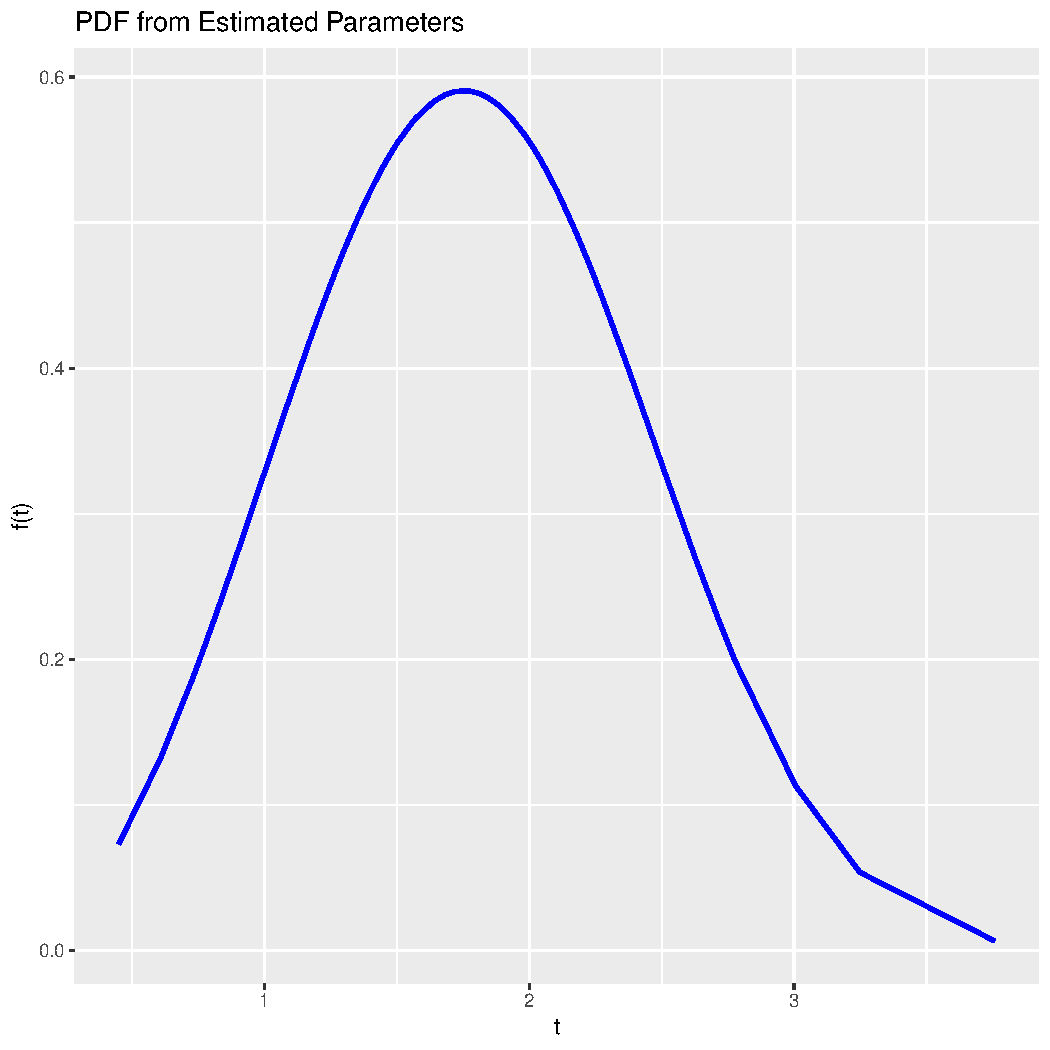
\includegraphics[width=\maxwidth]{figure/unnamed-chunk-17-1} 
\end{knitrout}

\newpage

\begin{knitrout}
\definecolor{shadecolor}{rgb}{0.969, 0.969, 0.969}\color{fgcolor}\begin{kframe}
\begin{alltt}
\hldef{df2} \hlkwb{<-} \hlkwd{data.frame}\hldef{(}\hlkwc{t} \hldef{= t_values,}
                  \hlkwc{St} \hldef{=} \hlnum{1} \hlopt{-} \hlkwd{pweibull}\hldef{(t_values,} \hlkwc{shape} \hldef{= alpha,}
                              \hlkwc{scale} \hldef{= lambda))}

\hldef{df2} \hlopt
  \hlkwd{ggplot}\hldef{(}\hlkwd{aes}\hldef{(}\hlkwc{x} \hldef{= t,} \hlkwc{y} \hldef{= St))} \hlopt{+}
  \hlkwd{geom_line}\hldef{(}\hlkwc{col} \hldef{=} \hlsng{'blue'}\hldef{,} \hlkwc{linewidth} \hldef{=} \hlnum{1}\hldef{)} \hlopt{+}
  \hlkwd{labs}\hldef{(}\hlkwc{x} \hldef{=} \hlsng{"t"}\hldef{,} \hlkwc{y} \hldef{=} \hlsng{"S(t)"}\hldef{,}
       \hlkwc{title} \hldef{=} \hlsng{"Survival Function from Estimated Parameters"}\hldef{)}
\end{alltt}
\end{kframe}
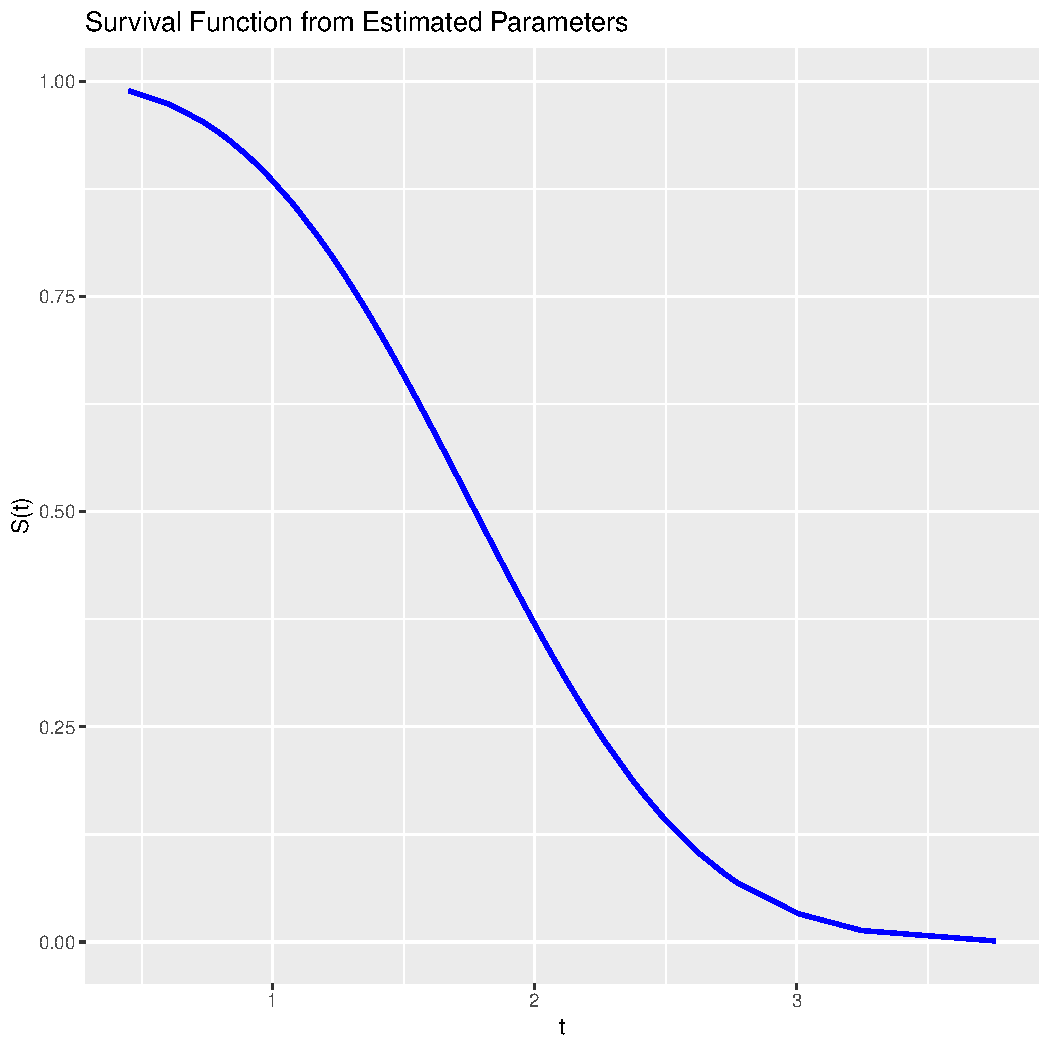
\includegraphics[width=\maxwidth]{figure/unnamed-chunk-18-1} 
\end{knitrout}

\newpage

\begin{knitrout}
\definecolor{shadecolor}{rgb}{0.969, 0.969, 0.969}\color{fgcolor}\begin{kframe}
\begin{alltt}
\hldef{df3} \hlkwb{<-} \hlkwd{data.frame}\hldef{(}\hlkwc{t} \hldef{= t_values,}
                  \hlkwc{ht} \hldef{= df1}\hlopt{$}\hldef{ft} \hlopt{/} \hldef{df2}\hlopt{$}\hldef{St)}

\hldef{df3} \hlopt
  \hlkwd{ggplot}\hldef{(}\hlkwd{aes}\hldef{(}\hlkwc{x} \hldef{= t,} \hlkwc{y} \hldef{= ht))} \hlopt{+}
  \hlkwd{geom_line}\hldef{(}\hlkwc{col} \hldef{=} \hlsng{'blue'}\hldef{,} \hlkwc{linewidth} \hldef{=} \hlnum{1}\hldef{)} \hlopt{+}
  \hlkwd{labs}\hldef{(}\hlkwc{x} \hldef{=} \hlsng{"t"}\hldef{,} \hlkwc{y} \hldef{=} \hlsng{"h(t)"}\hldef{,}
       \hlkwc{title} \hldef{=} \hlsng{"Hazard Function from Estimated Parameters"}\hldef{)}
\end{alltt}
\end{kframe}
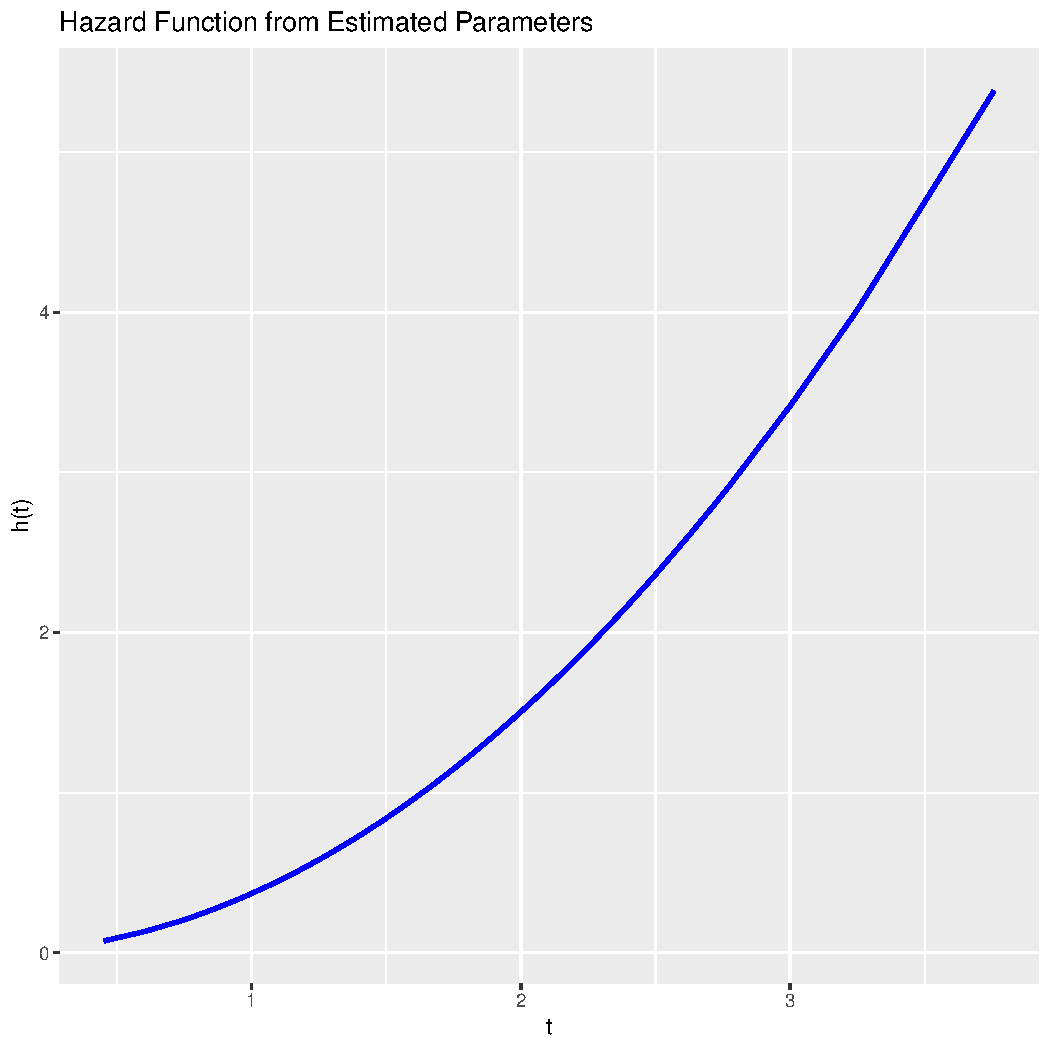
\includegraphics[width=\maxwidth]{figure/unnamed-chunk-19-1} 
\end{knitrout}

\newpage

\begin{knitrout}
\definecolor{shadecolor}{rgb}{0.969, 0.969, 0.969}\color{fgcolor}\begin{kframe}
\begin{alltt}
\hldef{df4} \hlkwb{<-} \hlkwd{data.frame}\hldef{(}\hlkwc{t} \hldef{= t_values,}
                  \hlkwc{Ht} \hldef{=} \hlopt{-}\hlkwd{log}\hldef{(df2}\hlopt{$}\hldef{St))}

\hldef{df4} \hlopt
  \hlkwd{ggplot}\hldef{(}\hlkwd{aes}\hldef{(}\hlkwc{x} \hldef{= t,} \hlkwc{y} \hldef{= Ht))} \hlopt{+}
  \hlkwd{geom_line}\hldef{(}\hlkwc{col} \hldef{=} \hlsng{'blue'}\hldef{,} \hlkwc{linewidth} \hldef{=} \hlnum{1}\hldef{)} \hlopt{+}
  \hlkwd{labs}\hldef{(}\hlkwc{x} \hldef{=} \hlsng{"t"}\hldef{,} \hlkwc{y} \hldef{=} \hlsng{"H(t)"}\hldef{,}
       \hlkwc{title} \hldef{=} \hlsng{"Cumulative Hazard Function from Estimated Parameters"}\hldef{)}
\end{alltt}
\end{kframe}
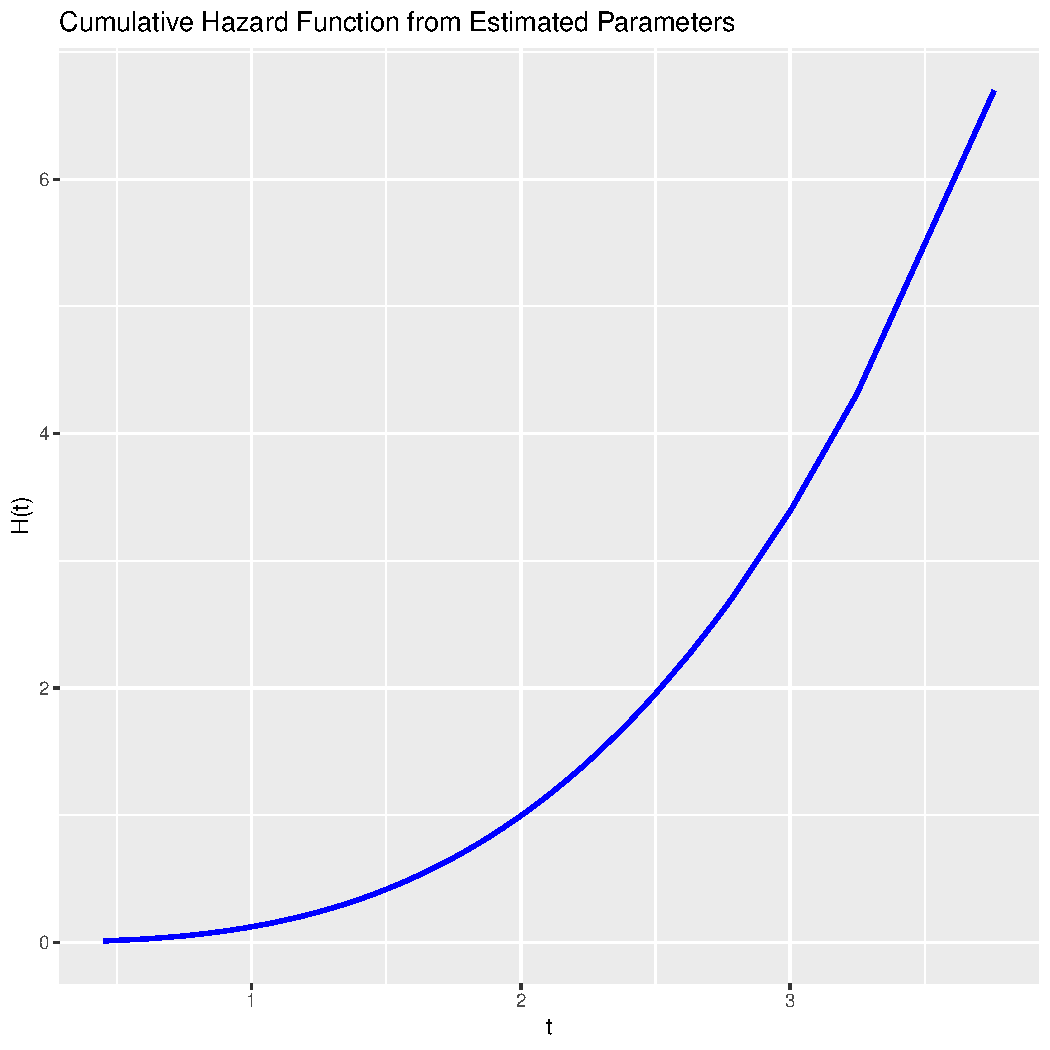
\includegraphics[width=\maxwidth]{figure/unnamed-chunk-20-1} 
\end{knitrout}
\end{document}
